\documentclass[12pt, twoside]{article}
\usepackage[letterpaper, margin=1in, headsep=0.5in]{geometry}
\usepackage[english]{babel}
\usepackage[utf8]{inputenc}
\usepackage{amsmath}
\usepackage{amsfonts}
\usepackage{amssymb}
\usepackage{tikz}
\usepackage{yhmath}
%\usetikzlibrary{quotes, angles}

\usepackage{graphicx}
\usepackage{enumitem}
\usepackage{multicol}

\usepackage{fancyhdr}
\pagestyle{fancy}
\fancyhf{}
\renewcommand{\headrulewidth}{0pt} % disable the underline of the header

\fancyhead[RE]{\thepage}
\fancyhead[RO]{\thepage \\ Name: \hspace{3cm}}
\fancyhead[L]{BECA / Dr. Huson / 10th Grade Geometry\\* 14 June 2019}

\begin{document}
\subsubsection*{13.10 Do Now: Mixed review}
 \begin{enumerate}

  \item In the diagram below, $\overline{AC}$ has endpoints with coordinates $A(-4,1)$ and $C(5,4)$.
   \begin{center} %4 quadrant regents grid
     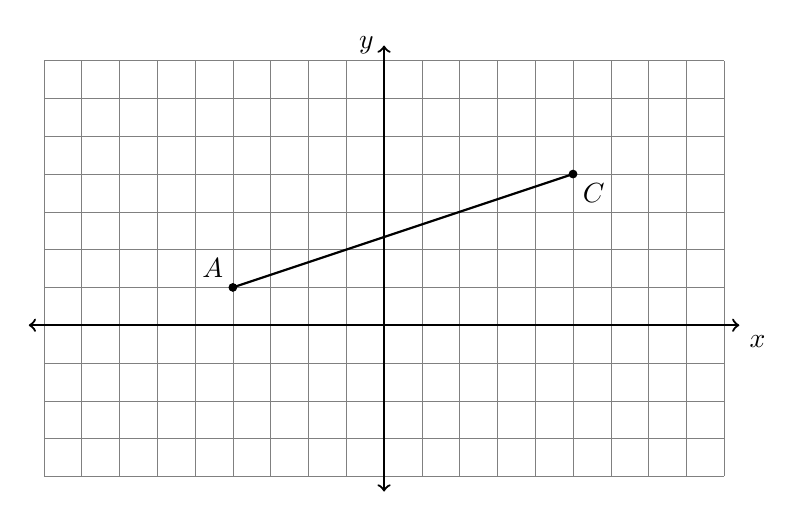
\begin{tikzpicture}[scale=.48]
       \draw [help lines] (-9,-4) grid (9,7);
       \draw [thick, <->] (-9.4,0) -- (9.4,0) node [below right] {$x$};
       \draw [thick, <->] (0,-4.4)--(0,7.4) node [left] {$y$};
       \draw [thick] (-4, 1)--(5,4);
       \draw [fill] (-4, 1) circle [radius=0.1] node[above left] {$A$};
       \draw [fill] (5, 4) circle [radius=0.1] node[below right] {$C$};
     \end{tikzpicture}
   \end{center}
   If $B$ is a point on $\overline{AC}$ and $AB{:}BC = 1{:}2$,  what  are  the coordinates of $B$? \vspace{4cm}

   \item The directed line segment $MN$ has endpoints $M(-3,-6)$ and $N(2,4)$. Point $P$ divides $\overline{MN}$ such that $MP {:}PN$ is $2{:}3$. What are the coordinates of $P$?\\[0.25cm]
   [Use the scrap Regents graph paper to help answer this problem] \vspace{4cm}

\newpage
  \item Triangle $ABC$ is dilated with a scale factor of $k$ centered at $A$, yielding $\triangle ADE$, as shown. Given $AB=9$, $BC=12$, $AC=14$, and $DE=16$. \\[0.25cm] Find $k$, $BD$, and $AE$ (the scale factor).\\[0.25cm]
     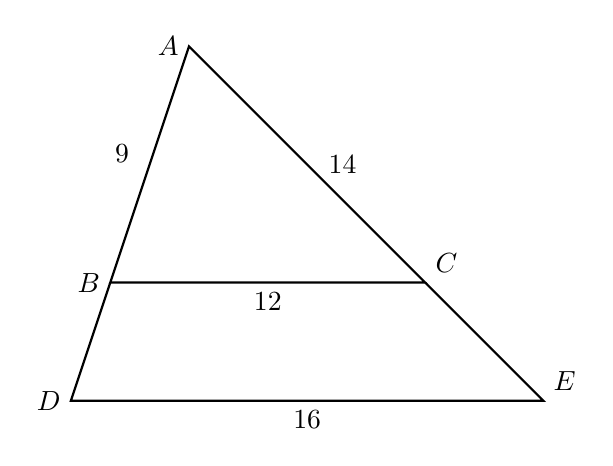
\begin{tikzpicture}[scale=0.5]
       \draw [thick]
       (0,0)node[left]{$B$}--
       (8,0)node[above right]{$C$}--
       (2,6)node[left]{$A$}--cycle;
       \draw [thick]
       (0,0)--
       (-1,-3)node[left]{$D$}--
       (11,-3)node[above right]{$E$}--(8,0);
       \node at (4,0)[below]{$12$};
       \node at (5.3, 3)[right]{$14$};
       \node at (0.3, 2.8)[above]{$9$};
       \node at (5,-3)[below]{$16$};
     \end{tikzpicture}
  \vspace{4cm}

  \item Given $\triangle ABP$ and $\triangle JKP$ as shown below. $\overline{AB} \parallel \overline{JK}$. $AP=5.7$, $JP=11.4$, and $JK=14.8$. Find $AB$.\\[0.5cm]
    \begin{tikzpicture}[scale=1.4]
        \draw [thick]
          (0.25,-1)node[right]{$B$}--
          (-0.5,2)node[left]{$K$}--
          (4,0)node[right]{$J$}--
          (0,0)node[above right]{$P$}--
          (-2,0)node[left]{$A$}--cycle;
      \end{tikzpicture}

\newpage
  \item What single transformation maps $\triangle ABC$ onto $\triangle DEF$, shown below? Fully specify the transformation.
    \begin{center}
      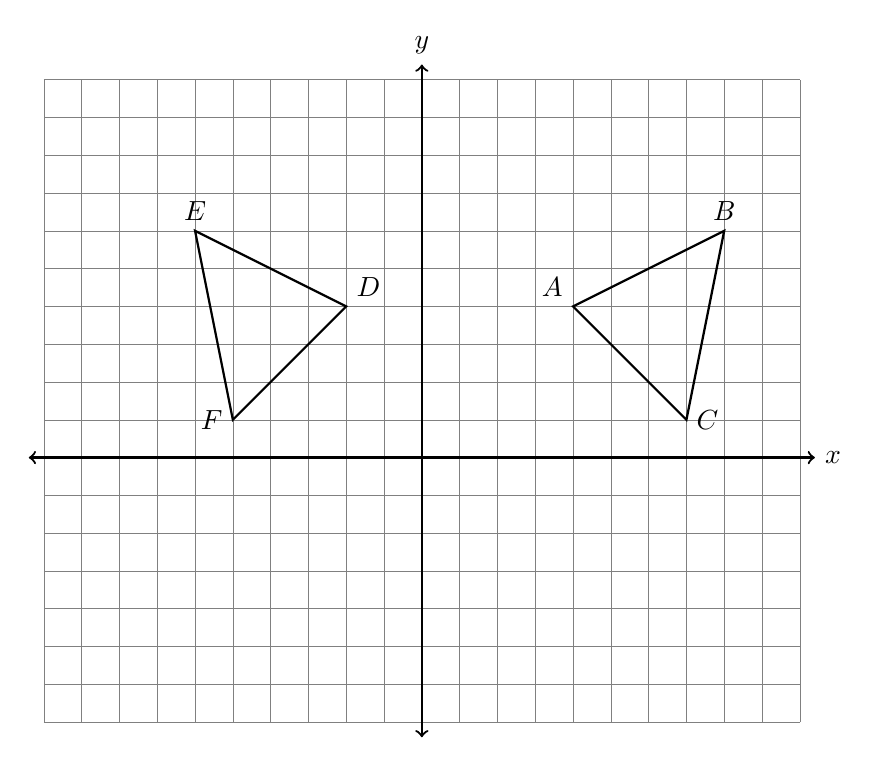
\begin{tikzpicture}[scale=.48]
        \draw [help lines] (-10,-7) grid (10,10);
        \draw [thick, <->] (-10.4,0) -- (10.4,0) node [right] {$x$};
        \draw [thick, <->] (0,-7.4)--(0,10.4) node [above] {$y$};
        \draw [thick]
          (4,4) node[above left] {$A$}--
          (8,6) node[above] {$B$}--
          (7,1) node[right] {$C$}--cycle;
        \draw [thick]
          (-5,1) node[left] {$F$}--
          (-6,6) node[above] {$E$}--
          (-2,4) node[above right] {$D$}--cycle;
      \end{tikzpicture}
    \end{center}

  \item Dilate the $\triangle PQR$ by a factor of $2$ centered at $(4,2)$, drawing its image $\triangle P'Q'R'$ and labeling its vertices.
    \begin{center}
      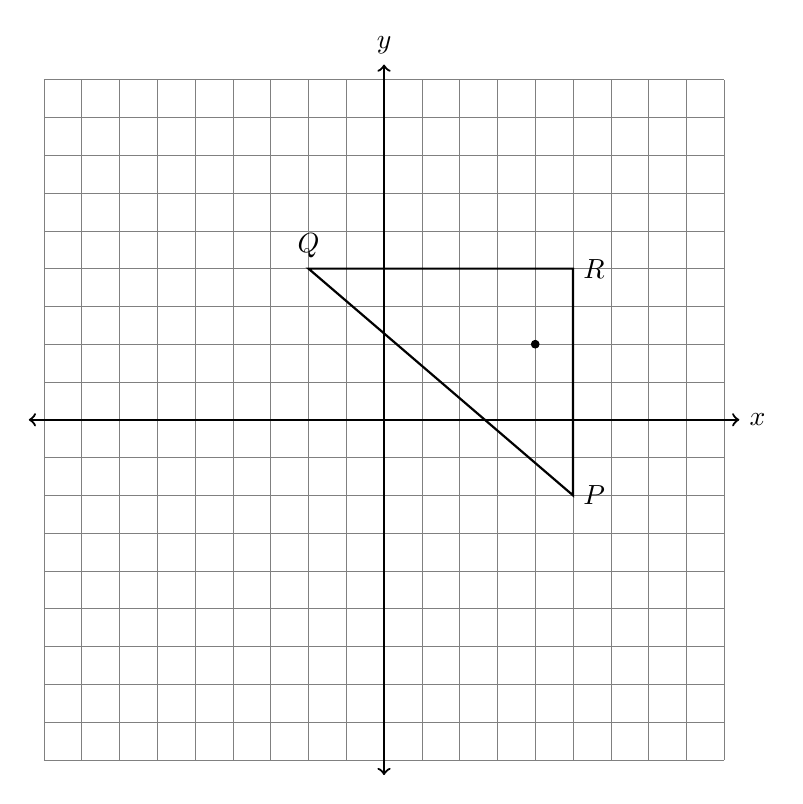
\begin{tikzpicture}[scale=.48]
        \draw [help lines] (-9,-9) grid (9,9);
        \draw [thick, <->] (-9.4,0) -- (9.4,0) node [right] {$x$};
        \draw [thick, <->] (0,-9.4)--(0,9.4) node [above] {$y$};
        \draw [thick]
          (5,-2) node[right] {$P$}--
          (-2,4) node[above] {$Q$}--
          (5,4) node[right] {$R$}--cycle;
        \draw [fill] (4,2) circle [radius=0.1];
      \end{tikzpicture}
    \end{center}

\newpage

  \item Write down the center and radius of the circle represented by
  $(x+1)^2+(y+3)^2=1$. \vspace{2cm}

  \item Write down the equation of a circle with radius $r=4$ and center $(7,-3)$. \vspace{2cm}

  \item Which equation represents a circle with radius $4$ centered at $(1,-2)$?
   \begin{enumerate}
     \begin{multicols}{2}
     \item   $x^2+2x + y^2-4y = 9$ \vspace{0.5cm}
     \item   $x^2-2x + y^2+4y = 9$
     \item   $x^2+2x + y^2-4y = 16$ \vspace{0.5cm}
     \item   $x^2-2x + y^2+4y = 16$
     \end{multicols}
   \end{enumerate} \vspace{4cm}

   \item Circle $O$ has a radius $AO=8$ cm, as shown below, and arc measure $m \wideparen{AB}=90^\circ$.
      \begin{multicols}{2}
        \begin{tikzpicture}[scale=.6]
          \draw (0,0) circle[radius=5];
          \draw [thick]
          (0:5) node[right] {$A$}--(0,0);
          \draw [thick] (0,0)--(90:5) node[above] {$B$};
          \fill (0,0) circle[radius=0.1] node[below]{$O$};
          \draw (35:6) node{$90^\circ$};
          \draw (0:2.5) node[below]{$8$};
          %\draw (75:1.8) node[above] {$C$};
          %\draw (290:5) node[below] {$D$};
        \end{tikzpicture}
      \columnbreak
        \begin{enumerate}
          \item Find the $m \angle AOB$. \vspace{1cm}
          \item Find the length of the arc $\wideparen{AB}$ to the \emph{nearest tenth}. \vspace{3cm}
          \item Find the area of the sector $AOB$ to the \emph{nearest tenth}. %\vspace{2.5cm}
        \end{enumerate}
      \end{multicols}

\end{enumerate}
\end{document}
